\chapter{Introduction}

\section{The Active Galactic Nuclei: Quasar vs. Radio Accretion Modes}
Active galaxies constitute a distinctive class characterized by an intensely energetic source at their center, known as an Active Galactic Nucleus (AGN). Since the first observation of an active galaxy in the early 1900s \cite{Shields_1999}, numerous studies have been conducted on this intriguing category of galaxies. To this day, efforts persist in unraveling the nature and role of active galaxies within the broader context of galactic formation and evolution.

Research in this field has demonstrated that the intense radiation must emanate from a compact region, with a spatial dimension not exceeding 100 parsecs. This estimation was derived from the temporal variability observed in some of these sources \cite{1959ApJ...130...38W}. Additionally, it has been noted that AGNs exhibit luminosity variations of over $50\%$ within timescales ranging from days to years. Such fluctuations can only be explained if a substantial portion of the emission region is randomly connected. These observations strongly imply that the central component of AGNs is a rapidly accreting Supermassive Black Hole (SMBH).

AGN emissions span the entire electromagnetic spectrum, each wavelength band offers insights into specific components and associated phenomena within AGN \cite{2017NatAs...1E.194P}. 

In addition to the central SMBH \cite{2006ApJ...652..216R} there is a disk of accreting matter onto it, that emits a significant amounts of ultraviolet (UV) radiation. Above this disk, a cloud of relativistic electrons is believed to be there \cite{2005ASPC..343..435K}. This cloud reprocess the UV photons emitted from the disk, re-emitting them at X-ray energy levels.
A population of clouds exists in close proximity to the SMBH, that is known as the Broad Line Region
(BLR), because the kinematics of these clouds are significantly affected by the gravitational pull of the SMBH, resulting in broader spectral lines. Beyond the BLR, there exists an outer region surrounding the SMBH known as the Narrow Line Region (NLR). In contrast to the BLR, the NLR is characterized by narrower spectral lines, indicating distinct physical conditions and dynamics. 
Additionally, surrounding the disk, there's a toroidal-shaped volume composed of a mixture of gas and dust, leading to the partial absorption of central radiation. The torus is the main component used from the “Unified Model” \cite{1995PASP..107..803U} to explain the existence of different populations of AGN. According to this model, different AGNs are the same population of objects with specific inclinations to our line-of-sight direction \cite{1993ARA&A..31..473A}.

In particular it is possible to distinguish :
 
\begin{itemize}
  \item \textbf{Type I:} For these types of AGN, broad emission lines, emitted from the BLR, with typical width in the range of in the range of $\sim 10^{3}$-$10^{4}$ $\text{km s}^{-1}$ exhibit a broad component,  along with narrow emission lines from the NLR. In this configuration, the observer is situated at a small angle relative to the torus axis, allowing the radiation from circumnuclear regions to remain unobscured along the line of sight.
  
  \item \textbf{Type II:} In this scenario, the spectrum of the AGN comprises solely narrow emission lines, not exceeding 1200 $  \text{km s}^{-1}$, due to the fact that the line of sight intersects the obscuring matter of the torus, obscuring the BLR.
  
\end{itemize}
A visual depiction of the Unified Model is shown in Fig.\ref{2}.

The energy released during the accretion process of a SMBH plays a significant role in shaping the evolution of the host galaxy \cite{2021A&A...646A.167M}. In this context, the literature often discusses positive and negative feedback mechanisms.
Positive feedback occurring when the AGN feedback promotes stellar formation, while negative feedback involves the suppression of star formation, respectively. Feedback from SMBH accretion is capable of heating diffuse gas \cite{2005Natur.433..604D} and depositing heavy elements across the extensive surrounding environment \cite{2000ApJ...539L..13G}, with effects observed at scales exceeding kpc scales. Two distinct AGN feedback mechanisms have been proposed, each associated with different rates of mass accretion onto the SMBH (e.g. \cite{2012ARA&A..50..455F, 2017NatAs...1E.165H}).

\begin{itemize}
	\item \textbf{QSO's Radiative Feedback :} This feedback mode, often referred as quasar mode, consists in a high accretion rate of the SMBH via an optically-thick and geometrically-thin disk, and most of the energy is released in form of radiation.
	\item \textbf{QSO's Radio Feedback :} In this scenario, the SMBH accretion of hotter gas happens with a low rate in a optically-thin and geometrically-thick disk configuration, releasing energy in form of relativistic particles such as Radio Jets.
\end{itemize}
%Check ok !!!
\begin{figure}[hbtb]
  \centering
  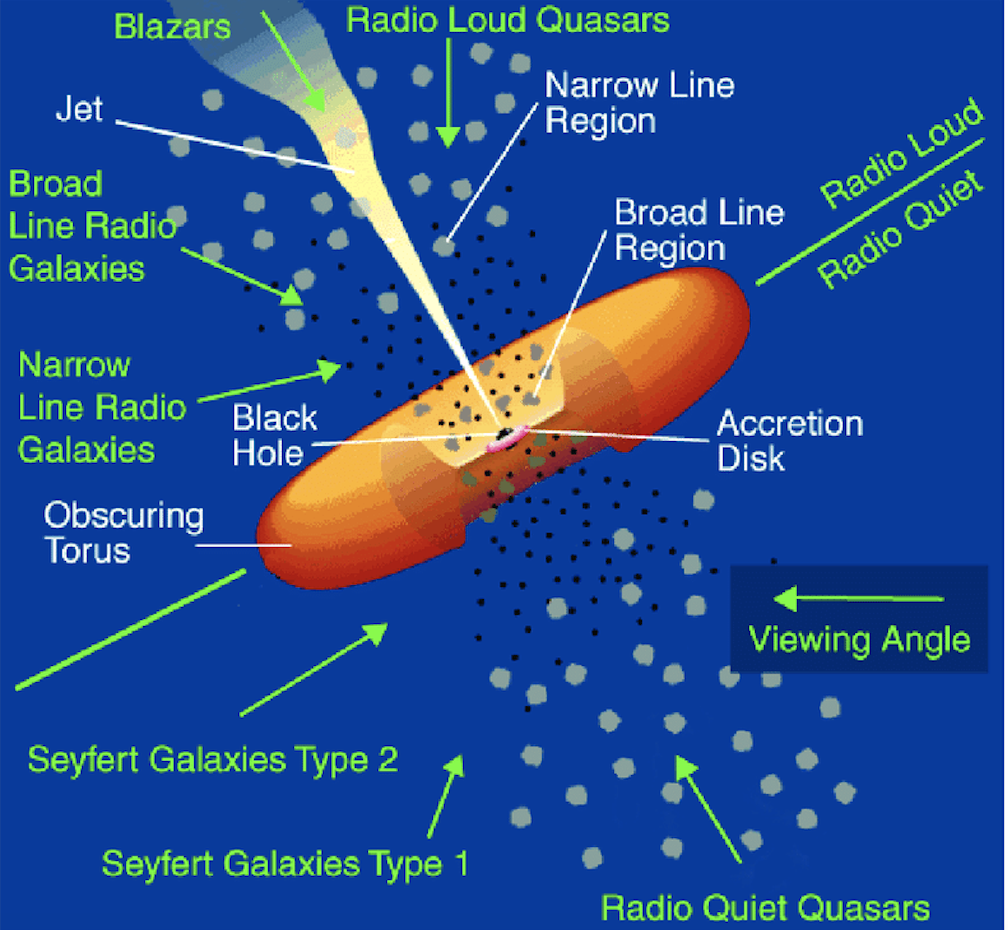
\includegraphics[width=0.5\textwidth]{UnifiedAGNmodel}
  \caption{The Unified AGN model as proposed in \cite{1995PASP..107..803U}, It elucidates AGN taxonomy by considering various viewing angles relative to the torus.}
  \label{2}
\end{figure}

\section{The Brightest Cluster Galaxies }
The Hierarchical Galaxy Formation Model stands as a cornerstone in our understanding of cosmic structure formation, delineating the principal pathways through which galaxies growth their stellar and gas mass assimilating matter from their surroundings \cite{1994MNRAS.271..781C}.

One of the most extreme examples in this context involves the study of Brightest Cluster Galaxies (BCGs), a unique class of galaxies, situated at the center and typically standing out as the most luminous and massive objects within the entire cluster.( e.g. \cite{2015MNRAS.448....2W} ). Considering their environment, observational studies, have indicated that the evolution of BCGs differs from the normal galactic path \cite{2020MNRAS.498.2719T}. As different studies have shown, BCGs' mass assembly is primarily influenced by dry mergers \cite{2007MNRAS.375....2D, 2019ApJ...881..150C}.

The majority of the BCGs are elliptical galaxies, but their properties deviate from established scaling relations for ellipticals. While most BCGs align with the Fundamental Plane, deviations, such as lower velocity dispersions and larger radii than predicted by the Faber–Jackson and Kormendy relations, have been observed (e.g \cite{1991ApJ...375...15O}). Recent findings suggest variations in these relations based on galaxy luminosity for all ellipticals. Additionally, BCG surface brightness profiles and radii depend on host cluster properties \cite{2005MNRAS.364.1354B}. 

\begin{comment}
Due to their distinct evolutionary histories, the primary mechanism driving the mass growth of galaxies is associated with cooling flows within lower mass halos at high redshifts.
However, at low redshifts, this phenomenon diminishes, primarily due to increased Active Galactic Nuclei ( AGN ) activity accreting mass into their typically hosted SMBH \cite{2006ApJ...652..216R}.
 \end{comment}
 
BCGs are mainly characterized by Radio Mode accretion of their SMBH, thus exhibiting radio loud emission as well as radio jets. As presented in \cite{2007MNRAS.379..867V} these relativistic jets of radio emission are also recognized as one of the main explanation of the so called "Cooling flow problem". 
While Theoretical expectations propose rapid cooling and gas flow toward the center, fostering new star formation, actual observations reveal a much slower cooling process, leading to the discrepancies.
The inclusion of radio jets provides a resolution to this issue by infusing energy into the Intracluster Medium (ICM), the hot gas within a galaxy cluster. This injection hinders the rapid cooling and collapse of gas toward the center, deviating from theoretical predictions. However observational studies found that temperature of cluster cores fails to fall below $\sim 30\%$ at large radii resulting in an amount of cooling gas corresponding only to the $\sim 10\%$ expected from the existent cooling flow model. \cite{David_2001} % OKOKOK

\newpage
\section{ Main Scientific Question of the Thesis} %Chiedere come mai ci distanziamo così tanto dalle scorse tesi
In this context, the main scientific question driving this work is to understand \textbf{whether the special evolution of BCGs, along with their dense environment, affects the accretion of SMBHs in their centers compared to other types of galaxies in the local universe}.

In particular, this study will present a comparative analysis between two representative samples of BCGs and Non-BCGs to highlight the substantial differences that the cluster environment induces in SMBH accretion.


To address this particular question, I conducted an analysis on a galaxy sample, the Sloan Digital Sky Survey Data Release 7 (SDSS DR7), as outlined in \cite{2009ApJS..182..543A}, and the C4 BCGs catalogue by Anja Von Der Linden and Best \cite{2007MNRAS.379..867V}. For these specific BCGs and non-BCGs sample, I utilized the common optical line fluxes ($H\alpha$, [OIII], $H\beta$, [NII], and [SII] doublets) provided by the Max Planck Institute for Astrophysics and Johns Hopkins University team to classify the galaxies hosting an AGN on the basis of the standard optical diagnostic diagram known as BPT \cite{1981PASP...93....5B}. Furthermore, through the cross-match between the aforementioned catalogs with datasets derived from NVSS and FIRST radio surveys, as outlined in \cite{2005MNRAS.362....9B}, I identified BCGs associated with radio loud emission, as an indication of the presence of radio mode SMBH accretion and a potential radio jet.

The analyses and the description of the data will be presented in the next chapter. 

%%%%% Apparentemente tutto corretto secondo le correzioni di Andrea 
